\documentclass[a4paper,12pt]{article}

\usepackage{amsfonts}
\usepackage{amssymb}
\usepackage{amsmath}
\usepackage{epsfig,graphicx}
\usepackage{color} 
\usepackage{calc}  % needed to count in enumerate with user-defined counter !!
\usepackage{verbatim}
\usepackage{pifont, wasysym}
\usepackage{multicol}
\usepackage{marvosym,wasysym}

%page layout
\setlength\oddsidemargin{0.0cm}
\setlength\evensidemargin{0.0cm}
\setlength\headsep{25pt}       
\setlength\textwidth{16cm}
\setlength\textheight{23cm}

\newcommand{\dinosaur}{\textbf{\epsfig{file=diplodocus.ps,width=4.8cm,height=3.75cm,angle=0}}}
\newcommand{\debiangnu}{\textbf{
\epsfig{file=debiancurl.eps,width=0.5cm,height=0.5cm,angle=0}/
\epsfig{file=gnu.eps,width=0.5cm,height=0.5cm,angle=0}}}

\newcommand{\terminal}{\texttt{user@linux:\textasciitilde \$ }}
\newcommand{\ipopt}{\textsc{Ipopt}\ }
\newcommand{\tbase}{\texttt{user@linux:\textasciitilde/}}

\newcommand{\cppad}{\textsc{CppAD}\ }
\newcommand{\dune}{\textsc{DUNE}\ }
\newcommand{\paraview}{\textsc{ParaView}\ }
\newcommand{\mpich}{\textsc{mpich}\ }
\newcommand{\opengl}{\textsc{OpenGL}\ }
\newcommand{\lapack}{\textsc{LAPACK}}
\newcommand{\blas}{\textsc{BLAS}\ }
\newcommand{\atlas}{\textsc{ATLAS}\ }

\newcommand{\cplusplus}{\texttt{C++}\ }
\newcommand{\fortran}{\textsc{FORTRAN}\ }

\newcommand{\dyeitred}{\textcolor{red}}{}
\newcommand{\dyeitblue}{\textcolor{blue}}{}
\newcommand{\dyeitgreen}{\textcolor{green}}{}

\begin{document}
\thispagestyle{empty}
\setlength{\parindent}{0pt}

\begin{center} \ \Huge{\textbf{\textsf{Installation of 3$^{\textbf{rd}}$-Party
  Software}}} 
\end{center}

This is a hands-on manual how to install the necessary software used for different model reduction approaches.\\
For my method, you need at least
\begin{itemize}
\item \lapack
\item UMFPACK
\item \cppad and
\item OpenMP.
\end{itemize}
If, in addition, optimization is involved, please install
\begin{itemize}
\item IPOPT and
\item MUMPS.
\end{itemize}
If you decide to run your applications on distributed systems, you need to install as well
\begin{itemize}
\item DUNE and
\item MPI.
\end{itemize}
In case you are running a Linux machine, some of the aforementioned tools should already be available for your distribution. If not, you may follow the installation instructions below. 

\medskip
\begin{center}
 \Large {\textbf{\textsf{Getting and using LAPACK}}}
\end{center}
Suppose you're using \debiangnu-Linux\footnote{cf. reference section if you're running a system which does not contain \lapack and so forth.}.
 
\newcounter{local1}\renewcommand{\labelenumi}
  {\setcounter{local1}{181+\value{enumi}}%
    \ding{\value{local1}}}
\begin{enumerate}
  \item Get the \atlas packages:
    \begin{center}
      \texttt{\# \ aptitude install libatlas3gf-base libatlas-base-dev libatlas3gf-sse2 libatlas-sse2-dev libatlas-doc libatlas-test libatlas-headers   }
    \end{center}
  \item Get the \blas packages:
    \begin{center}
      \texttt{\# \ aptitude install libblas-dev libblas-doc libblas-test libblas3gf }
    \end{center}
  \item Get the \lapack packages:
    \begin{center}
      \texttt{\# \ aptitude install liblapack-dev liblapack-doc liblapack-pic liblapack3gf scalapack1-mpich\dyeitgreen{\footnote{\dyeitgreen{This and the next one are quite optional and provide certain \textsc{MPICH} extensions.}}} scalapack-mpich-dev}
    \end{center}
\end{enumerate}

\dyeitred{\Stopsign \ Download the \texttt{-dev} files as well (they often contain new libraries or stuff needed for properly running linear algebra calculations!}

\medskip
\atlas, \blas and \lapack are now installed in \textit{/usr/lib} and \textit{/usr/include}.\\
You can change to the /usr/lib - directory and type \texttt{find liblapack.so.*} to check how the shared libraries are named (normally they should be called \textit{liblapack.so.3gf, liblapack.so.3gf.0} and the like).


\medskip
\begin{center}
 \Large {\textbf{\textsf{A toy example}}}
\end{center}
Assume you want to solve the following tridiagonal linear system
\begin{equation}
  \label{linsys}
 \begin{bmatrix}
    2  & -1 &  0 & 0 &  0 \\
    -1 &  2 & -1 &  0 &  0\\
    0  & -2 & 3  &-1 &  0 \\
    0  & 0  &-1  & 3  &-2  \\
    0   &0 & 0   & -1 & 1 
\end{bmatrix}
\cdot 
\begin{bmatrix} x_0\\ x_1\\ x_2\\x_3\\x4\end{bmatrix}
= \begin{bmatrix} 1\\ 2\\ 3\\2\\1\end{bmatrix}.
\end{equation}

Clearly, the solution is given by
\begin{equation*}
  x^* = [x_0, x_1, x_2, x_3, x_4]^{T} =
  \begin{bmatrix} 6.5\\ 12.0\\ 15.5\\19.5\\20.5\end{bmatrix}.
\end{equation*}

The linear algebraic system (\ref{linsys}) may now be implemented in \texttt{C++} with the help of \lapack in a very simple manner 
\verbatiminput{simplelapack.cc}


\medskip
\dyeitred{\Stopsign \ \begin{itemize}
 \item Do NOT forget to specify an extern linkage convention via \texttt{extern "C"\{\ldots \}\footnote{\dyeitred{Otherwise an error occurs, like "\texttt{error: ‘...dgtsv\_ was not declared in this scope}" or "\texttt{...(.text+0x9a): undefined reference to `dgtsv\_(long const*, long const*, double*, double*, double*, double*, long const*, long*)'
collect2: ld returned 1 exit status}".}}}.
 \item Do NOT forget the underscore '\_' after the \fortran function name inside the  \texttt{extern "C"} environment (i.e. \texttt{dgtsv\_(\ldots)} and \underline{not} only \texttt{dgtsv(\ldots)})!
  \end{itemize}
}

\smallskip
\textbf{Note:} If you want to retain a once calculated solution of system (\ref{linsys}) without being destroyed by the next call of \textit{tridiagsyssolver}, simple add \texttt{static} in front of the return value of \textit{tridiagsyssolver}
(here it would read \texttt{static long  tridiagsyssolver(\ldots)}).
\medskip
\begin{center}
 \Large {\textbf{\textsf{How do I compile and link the program?}}}
\end{center}
That's rather easy. Let's say the above program is called "simplelapack.cc". Just type
\begin{center}
  \texttt{ c++ -o simplelapack simplelapack.cc  -llapack -lblas -lg2c -lm}
\end{center}
Sometimes, especially in a Makefile one has to add \dyeitred{\texttt{-L/usr/lib/liblapack.so.3gf}}\ .

\smallskip
Any hidden mistakes? Run \texttt{valgrind --leak-check=full ./simplelapack}

\smallskip
As a matter of fact, the above programme is completely independent of the \atlas libraries. If the optimized \atlas versions are present it will use them, if they are absent the reference implementation will be used instead.  

\begin{center}
 \dinosaur
\end{center} 

\medskip
\begin{center}
 \Large {\textbf{\textsf{Installation of Ipopt}}}
\end{center}


\newcounter{local}\renewcommand{\labelenumi}
  {\setcounter{local}{181+\value{enumi}}%
    \ding{\value{local}}}
\begin{enumerate}
\item Download the \texttt{Ipopt} sources\footnote{\dyeitred{\texttt{Ipopt} needs the
  extern linear solver \texttt{MA27} and/or \texttt{MA57}. You have to
  register at \\ \texttt{http://www.cse.clrc.ac.uk/nag/hsl/} in order to get
  them ! Once you've got 'em, copy the \textit{*.f} files into
  \textit{~/SOFTWARE/Ipopt-version/ThirdParty/HSL} and proceed as described above\ldots}} from \begin{center}
  \texttt{http://www.coin-or.org/download/source/Ipopt/}
 \end{center}
\item Create a new directory in your home directory, say\begin{center}
  \texttt{\terminal mkdir SOFTWARE}
 \end{center} 
  \item Move the stuff to the newly created directory:
 \begin{center} 
 \texttt{\terminal mv  Ipopt-\textit{version}.tgz SOFTWARE}
  \end{center} 
  where from here and now on -\textit{version} denotes the version you have
  decided to download !
\item Change to the newly created directory, extract the files from
   the downloaded file, change to the extracted directory
   \textit{Ipopt-\textit{version}}, then create directory
   \textit{build} and change to this dir: 
  \begin{center}
   \begin{tabular}{l}
   \texttt{\terminal cd SOFTWARE}\\
   \texttt{\tbase SOFTWARE\$ gunzip Ipopt-\textit{version}.tgz}\\
   \texttt{\tbase SOFTWARE\$ tar xvf Ipopt-\textit{version}.tar}\\
   \texttt{\tbase SOFTWARE\$ cd Ipopt-\textit{version}} \\
   \texttt{\tbase SOFTWARE/Ipopt-\textit{version}\$ mkdir build; cd build}
    \end{tabular}
   \end{center} 
 \item \textbf{Alternative download:} Get current version via svn: \begin{center} \texttt{svn co https://projects.coin-or.org/svn/Ipopt/stable/\textit{version}\textvisiblespace CoinIpopt} \end{center} 
\item For getting further external software which can be used in conjunction with \ipopt, change to \textit{ThirdParty} and run in every subdirectory the \texttt{get.*} script.
 \item Creating \textit{build} is \underline{optional}. Nevertheless they advise to do so
     and to compile the stuff in that separate subdirectory (\dyeitred{Make sure the linear solvers MA27 and MC19 have been copied to \texttt{\tbase SOFTWARE/Ipopt-\textit{version}/ThirdParty/HSL}}): \texttt{../configure; make; make test; make install} and the installation can be found in  \texttt{\tbase SOFTWARE/Ipopt-\textit{version}/build}.\\
However, since we want to install \ipopt \textbf{globally}, e.g. in
\textit{/usr/local/}, we do \underline{not} change to \textit{build}, but stay
in the present directory (see prompt line in order to avoid confusion!). Next
configure the stuff into the desired installation path and compile it via \textit{make}:
       \begin{center}
      \begin{tabular}{l}
      \texttt{\tbase SOFTWARE/Ipopt-\textit{version}\$ ./configure --prefix
         /usr/local/  } \\
      \hspace{7.5cm} \texttt{\dyeitred{--with-lapack="-L/usr/lib -llapack"}}\\
       \texttt{\tbase SOFTWARE/Ipopt-\textit{version}\$ make}
       \end{tabular}
       \end{center}
The \texttt{./configure} script should terminate with \texttt{Main configuration of Ipopt successful}\\
   Note that the \textit{--with-lapack} flag (and often also the corresponding \textit{--with-blas="-L/usr/lib -latlas"} flag has to be set if you use your linux libraries instead of the $3^{\textrm{rd}}-$party versions provided by \ipopt. 
%\newpage
\item Test  compilation via \begin{center}
  \texttt{\tbase SOFTWARE/Ipopt-\textit{version}\$ make test}\end{center} The
  output to screen should look somehow like the following:\\
  \texttt{Testing AMPL Solver Executable...\\
  no AMPL solver executable found, skipping test...\\ Testing C++ Example...\\Test passed! \\ Testing C Example...\\Test passed!\\Testing Fortran Example...
    \\ Test passed!} 

\smallskip
\texttt{AMPL} does not interest me because it is non-free \smiley
\item Installation: \texttt{make install}
%% \item Change to root, if necessary, to finally install \ipopt globally.
%% \begin{center}
%%  \begin{tabular}{l}
%%    \texttt{\tbase SOFTWARE/Ipopt-\textit{version}\$ su}\\
%%    (now enter the root password)\\
%%    \texttt{\tbase SOFTWARE/Ipopt-\textit{version}\# make install}
%%  \end{tabular}
%% \end{center}
\item Add the following to your \textit{./bashrc}:\begin{center} \texttt{export LD\_LIBRARY\_PATH=\$LD\_LIBRARY\_PATH:/home/mfein/SOFTWARE/CoinIpopt/build/lib/} \end{center}
so that \texttt{Ipopt}'s runtime libraries can be detected.
\end{enumerate}
Now \ipopt has been installed globally and the source files and header files respectively can
be found in \textit{/usr/local/include/coin}. Binaries are in
\textit{/usr/local/lib}, e.g. \textit{libipopt.so}, etc.\\
For later use you can always use the Ipopt makefile which is automatically
delivered and lies in \textit{\textasciitilde/SOFTWARE/Ipopt-\textit{version}/Ipopt/examples/hs071\_cpp}

\medskip
\dyeitred{Uninstalling \ipopt:}
\begin{center}
   \begin{tabular}{l}
     \texttt{\tbase SOFTWARE/Ipopt-\textit{version}\$ su <enter passwd>}\\
     \texttt{\tbase SOFTWARE/Ipopt-\textit{version}\$ make uninstall}
   \end{tabular}
\end{center}

\begin{center}
 \dinosaur
\end{center} 
 
%\newpage
\begin{center}
 \Large {\textbf{\textsf{Installation of CppAD}}}
\end{center}

\newcounter{loc1}\renewcommand{\labelenumi}
  {\setcounter{loc1}{181+\value{enumi}}%
    \ding{\value{loc1}}}
\begin{enumerate}
\item Download the sources from 
 \begin{center}
   \texttt{http://www.coin-or.org/CppAD/Doc/installunix.htm}
\end{center}
Here you can download the stuff under \textit{Unix Tar Files}.
\item Assume that you've already created a dir called \textit{SOFTWARE} for
  3rd Party Software. Furthermore, assume also you have created a dir called
  \textit{CppAD} therein. Then simply copy the sources to there and extract them:
  \begin{center}
   \begin{tabular}{l} 
   \texttt{\tbase SOFTWARE/CppAD\$ tar -xvzf
     cppad-\textit{version}.\textit{license}.tgz}\\
     \texttt{\tbase SOFTWARE/CppAD\$ cd cppad-\textit{version}}\\
     (You can see if everything o.k. by checking \textit{cppad-\textit{version}/cppad/cppad.hpp}) 
     \end{tabular}
\end{center}

\item \underline{Also possible:} If you don't want to install \cppad simply copy the dir \textit{cppad} to
  your desired location and, later on, include it in your makefile via
  \textit{-I./} (assumed \textit{cppad} is a subdirectory therein !). 
  
 \item \textbf{Global installation:} Otherwise enter the extracted directory and configure \cppad in
   accordance with, e.g., \ipopt (under assumption that \ipopt's headers are
   installed somewhere, for instance in \textit{/usr/local/include/coin}:
   \begin{center}
     \texttt{\tbase SOFTWARE/CppAD\$ cd cppad-\textit{version}/; ./configure
       --prefix=/usr/local  --with-Documentation --with-Example --with-Speed
       --with-Introduction\dyeitred{\footnote{\dyeitred{\cppad says you can compile it
           also with \ipopt (provided \ipopt has been installed before),
           i.e. \texttt{IPOPT\_DIR=IpoptDir} has to be chosen such that
           \textit{IpoptDir/include/IpIpoptApplication.hpp} is a valid
           reference to the file \textit{IpIpoptApplication.hpp}.}}}}
    \end{center}
   \Stopsign Mind that only \textit{./configure} is mandatory. All additional
   strings are merely optional and serve to include examples that can be
   tested after \textit{make} has been invoked. Likewise the \cppad -
   documentation will be installed in subdirs of the directory specified by
   the \textit{prefix} string!\\
   \Stopsign Mind to write \textit{/usr/local} anywhere (if you use additional
   strings with \textit{./configure}) instead of
   \textit{/usr/local\textbf{/}} (i.e. omit forward slash character '/' !!)
 \item Compile stuff 
   \begin{center}
     \texttt{\tbase SOFTWARE/CppAD/cppad-\textit{version}\$ make}
     \end{center}
  \newpage
  \item \underline{Optional}: Test included examples, for instance, check the
    \textit{get\_started.cpp} example where the derivative of a polynomial of
    degree 4 with all coefficients being equal to 1, i.e. $f'(x) = 4x^3+3x^2+2x+1$ is evaluated at $x = 3$\\ Check
    \texttt{http://www.coin-or.org/CppAD/Doc/get\_started.cpp.htm} for further
    details:
    \begin{center}
   \begin{tabular}{l} 
     \texttt{\tbase SOFTWARE/CppAD/cppad-\textit{version}\$ cd
       introduction/get\_started}\\
     \texttt{\$\footnote{\texttt{\tbase
           SOFTWARE/CppAD/cppad-\textit{version}/introduction/get\_started\$
           is abbreviated by $\$$}} make; ./get\_started}
        
   \end{tabular}
    \end{center}
  should return '\texttt{f'(3) computed by CppAD = 142}'.

  \item Install it, hunk
    \begin{center}
 \begin{tabular}{l}
   \texttt{\tbase SOFTWARE/CppAD/cppad-\textit{version}\$ su}\\
   (now enter the root password)\\
   Then install it ('\#' is my abbreviation for the root mode in the present directory)\\ \texttt{\# make install}
 \end{tabular}
\end{center}
\end{enumerate}

Yet again, all the \cppad source files are installed globally in
\textit{/usr/local/include/cppad} and there should be no need to copy the
directory to every project you're programming \smiley

\begin{center}
 \dinosaur
\end{center} 


\newpage
\begin{center}
 \Large {\textbf{\textsf{Preparation of METIS}}}
\end{center}
\dyeitred{\Stopsign Install it from the scratch! In particular, don't copy a patched version ;) Otherwise you might get errors like ``undefined references to \_\_log2'', etc.}
\begin{enumerate}
\item Get METIS \begin{center} \texttt{http://glaros.dtc.umn.edu/gkhome/metis/metis/download} \end{center}
\item \texttt{tar xzvf metis-version.tar.gz} 
\item For \texttt{metis-4.0} you'll need the following patch \begin{center} \texttt{http://www.math-linux.com/IMG/patch/metis-4.0.patch} \end{center}
\item \texttt{cp metis-4.0.patch metis-4.0/}
\item \texttt{cd metis-4.0/; patch -p1 < metis-4.0.patch}
\item \texttt{make}
\end{enumerate}


Upon successful completion you should have some executables, namely \textit{graphchk, kmetis,  mesh2dual,mesh2nodal, oemetis, \ldots }.
%% \begin{center}
%%  \dinosaur
%% \end{center} 

\medskip
\begin{center}
 \Large {\textbf{\textsf{Installation of MUMPS}}}
\end{center}
After having installed METIS, we proceed as follows:
\begin{enumerate}
\item Get MUMPS from \begin{center} \texttt{http://graal.ens-lyon.fr/MUMPS/index.php?page=dwnld} \end{center}
\item \texttt{tar xzvf MUMPS\_version.tar.gz} 
\item \texttt{cd MUMPS\_version}
\item Edit \texttt{Makefile.inc} and change the following variables accordingly
\begin{itemize}
  \item \texttt{LMETISDIR = \$(HOME)/Sourcepath2Metis\footnote{\textit{``Sourcepath2Metis'' is a placeholder for your path to METIS}}/metis-4.0}
  \item \texttt{FC = gfortran}
  \item \texttt{FL = gfortran}
  \item Some compilers don't support the \texttt{-nofor\_main} optimized
    option. Just uncomment all occurances of it in in \textit{Makefile.inc}.
\end{itemize}
\item \texttt{make clean; make}
\end{enumerate}
Upon successful completion, you should find the following files in \textit{MUMPS\_version}: \textit{examples,lib,libseq, src}.
\begin{center}
 \dinosaur
\end{center} 


\medskip
\begin{center}
 \Large {\textbf{\textsf{Installing UMFPACK}}}
\end{center}
\dyeitred{\Stopsign UMFPACK requires BLAS and LAPACK ;)}
\begin{enumerate}
\item Get the following current packages needed in conjunction with UMFPACK:
\small{
\begin{itemize}
\item \texttt{http://www.cise.ufl.edu/research/sparse/umfpack/current/}
\item \texttt{http://www.cise.ufl.edu/research/sparse/SuiteSparse\_config/current/}
\item \texttt{http://www.cise.ufl.edu/research/sparse/amd/current/} 
\end{itemize}
}
\item Copy them into the \emph{same} directory
\item Unpack the above packages via \begin{center}\texttt{tar xzvf UMFPACK.tar.gz} \end{center} etc. 
\item \texttt{cd SuiteSparse\_config} \begin{itemize} \item Edit \textit{SuiteSparse\_config.mk}: \item comment line 184, i.e. \texttt{\#UMFPACK\_CONFIG} \item UNcomment line 187, i.e. write \texttt{UMFPACK\_CONFIG = -DNCHOLMOD} to use the whole thing without CHOLMOD \end{itemize}
\end{enumerate}


\newpage
\begin{center}
 \Large {\textbf{\textsf{Installation of DUNE}}}
\end{center}

Note that \dune depends on several packages which all have to be obtained
first.\\
Therefore I subdivide this section into several others explaining briefly the crucial
steps of their installation.

\medskip
\begin{center}
 \large {\textbf{\textsf{ParaView -- a fancy package for visualizing data}}}
\end{center}

\dyeitred{\Stopsign \ If you are using \textsc{Debian/GNU Linux} then you can simply ignore steps \ding{182} - \ding{186}!!! \\ Instead switch to root on command line (\texttt{su} \textit{enter root passwd...}) and type \newline \hspace{1.5cm} \texttt{\# aptitude install paraview } \\ That's it :-). }

\medskip
However, if you're the poor guy who is running \textsc{SuSe}, you must stick to the following steps: 
Install the sources of the
package \paraview from 
\begin{center}
\texttt{http://www.paraview.org/paraview/resources/software.html}
\end{center}
The sources are at the end of the \textit{Latest release  (x.y.z)} list, closely
followed by the Data sources (also beneficial, I suppose). \\

\newcounter{loc2}\renewcommand{\labelenumi}
  {\setcounter{loc2}{181+\value{enumi}}%
    \ding{\value{loc2}}}
\begin{enumerate}
\item A good installation guide (UNIX) is available from 
  \begin{center}
    \texttt{http://www.paraview.org/Wiki/ParaView:Build\_And\_Install\#On\_Unix-like\_systems}
    \end{center}
  \item Prerequisites: \\
    \begin{enumerate}
      \item \texttt{cmake} (version $\geq 2.4.5$):
       \begin{center}
         \begin{tabular}{l} 
           \texttt{cd \$HOME}\\
            \texttt{wget http://www.cmake.org/files/v2.4/cmake-2.4.5.tar.gz}\\
            \texttt{tar xvfz cmake-2.4.5.tar.gz}\\
            \texttt{mkdir cmake-2.4.5-bin}\\ 
             \texttt{cd cmake-2.4.5-bin}\\
            \texttt{../cmake-2.4.5/bootstrap --prefix=\$HOME/software}\\
            \texttt{make; su}\\
            \texttt{make install}


         \end{tabular}
       \end{center}
 O.k. now \texttt{cmake} is on your system\ldots

    \item Trolltech's \texttt{Qt qmake} (version
    $4.3.5$ recommended \Stopsign Stick to this version like the eye to the
    appearance of a beautiful woman (like with pretty women, other versions aren't
    supported yet!!)
    \begin{enumerate}
      \item Download, e.g. \textit{qt-x11-opensource-src-4.3.5.tar.gz} from
       \begin{center} 
        \texttt{ftp://ftp.trolltech.no/qt/source/}
       \end{center}
    \item Install it by following the manual which is available on 
    \begin{center}
      \texttt{http://doc.trolltech.com/4.3/install-x11.html}
    \end{center}
   \newpage
   \item Suppose again we have a directory \textit{SOFTWARE/Qt} to which the
      sources have been downloaded. Extract them via
       \begin{center}
         \begin{tabular}{l} 
            \texttt{cd SOFTWARE/Qt}\\
           \texttt{gunzip qt-x11-opensource-src-4.3.5.tar.gz}\\ 
            \texttt{tar xvf qt-x11-opensource-src-4.3.5.tar}
         \end{tabular}
       \end{center}
        Now the package directory \textit{qt-x11-opensource-src-4.3.5} is
        revealed. Change to it and build it 
          \begin{center}
         \begin{tabular}{l} 
           \texttt{cd qt-x11-opensource-src-4.3.5}\\
           \texttt{./configure}\\
           (automatically configures in
           \textit{/usr/local/Trolltech/Qt-4-3.5}. \\If you like change it via
           the prefix option but I use the default dir \\(like for the other
           software)). \\You are ask to accept the license, type \texttt{yes} \\
           (for reconfiguring, type \textit{make confclean; configure}\\ 
           \texttt{make}\\
            \texttt{su}\\
           (enter root password)\\
            \texttt{make install}
            \end{tabular}
       \end{center}
     \item \Stopsign Don't forget to set the environment variable for qmake in
       the file \textit{\$HOME/.profile} !!!:
       \begin{center}
         \begin{tabular}{l} 
          \texttt{PATH=/usr/local/Trolltech/Qt-4.3.5/bin:\$PATH}\\
          \texttt{export PATH}
            \end{tabular}
       \end{center}
\end{enumerate}    
 
%\end{enumerate}
That's it -- \textsc{Qt} is installed and ready to use \smiley
\item \dyeitred{Installing MPI such as \mpich}\\
This is an important issue, I fancy,  not only for \textsc{ParaView} since every
scientific software relies on it sooner or later.
 \begin{enumerate} 
 \item Download "UNIX (all flavors)" sources \textit{mpich.tar.gz} from
 \begin{center}
  \texttt{http://www.mcs.anl.gov/research/projects/mpi/mpich1/download.html}
   \end{center}
 
\item Choosing the correct devices and release, e.g. for \\
   \textbf{Workstations networks, Beowulf Clusters and Individual
     Workstations}: \textit{ch\_p4} (most general device, supports SMP nodes,
   MPMD programs, heterogeneous collections of systems,
   etc. This should suffice for most applications and is installed by default
   if you don't specify any device flags (cf. below) !) and  \textit{ch\_p4mpd}
   (only for homogeneous clusters)\\
   \textbf{Symmetric Multiprocessors (SMPs)}: \textit{ch\_shmem}\\
Fortunately, both configurations and installations are the \underline{same} ! (except for
\textit{ch\_p4mpd} where a special configure flag should be used).
 The installation guides can be found as PDF or PS files at the very bottom of the
   page.\\
   \textbf{Hint:} \texttt{uname -a} gives you some general information about your system
   which may be useful.
\item \textbf{Note:} Depending on how you want to calculate later on, it is
  useful to install remote shell \textit{rsh} as well as \textit{rsh-server} in advance and
  enable it via the following commands executed in root mode:
  \begin{center}
    \begin{tabular}{l}
      \texttt{\# chkconfig xinetd on}\\
      \texttt{\# chkconfig rsh on}\\
      \texttt{\# chkconfig rexec on}\\
      \texttt{\# chkconfig rlogin on}\\
      \texttt{\# service xinetd restart}
    \end{tabular}
  \end{center}
Now you should be able to run rsh via, e.g. \texttt{rhs localhost} which, when
executed, asks for your system password (like ssh would do).
  \item Run the set of commands \begin{center}
         \begin{tabular}{l} 
           \texttt{cd SOFTWARE; mkdir MPICH; cd MPICH}\\
           (assume you have copied the \mpich sources to this dir)\\
           \texttt{tar zxovf mpich.tar.gz}\\
           \texttt{cd mpich-1.2.7p1}
           
         \end{tabular}
         \end{center}
        %\newpage  
  \item For security reasons it seems advisable to configure \textsc{MPICH}
    with ssh. To avoid tedious password inputs, all logins to slaves should be
    made password-free:
    \begin{itemize}
      \item Generate \dyeitred{\underline{one}} ssh key via \texttt{ssh-keygen -r rsa}
        \item (Optional if no \textit{.ssh} dir exists on host you want to log
          in without password later on: \texttt{ssh targethost mkdir -p .ssh
            <enter targethost's passwd>)}
          \item \texttt{cat .ssh/id\_rsa.pub | ssh targethost 'cat >>
            .ssh/authorized\_keys'}
            \item \texttt{<enter targethost's passwd one last time\ldots>}
    \end{itemize}
    where \textit{targethost} denotes \underline{any} host you want to compute
    on (i.e. one ssh key suffices for all hosts)! In other words, simply execute the very last command for every user a on machine A (a@A) to user b on machine B (b@B).  
  
  \item Configure it via
               \begin{center}
                   \texttt{./configure \dyeitred{-rsh=ssh}\footnote{You can
                       also specifiy special \textsc{MPICH} devices via
                       \texttt{--with-device=ch\_shmem}. The \texttt{-rsh=ssh}
                     seems deprecated. By default it was substituted
                     automatically by some flag \texttt{RSHCOMMAND \ldots} } --prefix=/usr/local/mpich-1.2.7 2>\&1 | tee c.log}
               \end{center}
         from the dir of the \textsc{MPICH} sources,
         e.g. \textit{SOFTWARE/MPICH/mpich-1.2.7}. You need not to create dir \textit{/usr/local/mpich-1.2.7}. It will be
         created automatically during installation.
             \item \texttt{make 2>\&1 | tee make.log}
         \item \texttt{su; \textit{(enter password)}}
          \item \texttt{make install} 
            (to uninstall, run the script \textit{/usr/local/mpi-1.2.7/sbin/mpiuninstall})
   \item \dyeitred {\Stopsign Don't forget to set the environment paths in the file
     \textit{.bashrc} and/or \textit{.profile}} as follows:
     \begin{center}
      \begin{tabular}{l}
       \texttt{export
         LD\_LIBRARY\_PATH="\$LD\_LIBRARY\_PATH:/usr/local/mpich-\textit{version}/lib"}\\
        \texttt{export MANPATH="\$MANPATH:/usr/local/mpich-\textit{version}/man"}\\
        \texttt{export PATH="\$PATH:/usr/local/mpich-\textit{version}/bin"}
     \end{tabular}
     \end{center}


\end{enumerate}
 

 Now \mpich is installed in \textit{/usr/local/mpich-1.2.7}.\\ You can run test
  examples (cf. PDF guide) which I recommend !!! Change to the directory where
  the extracted \textsc{MPICH} sources are,
  e.g. \\ \textit{\$HOME/SOFTWARE/MPICH/mpich-1.2.7/}\\ Then again change to some
  subdirs therein, namely
  \begin{center}
    \begin{tabular}{l}
      \texttt{\$ cd examples/basic/}\\
      \texttt{\$ make clean; make cpi; ../../bin/mpirun -np 4 cpi} 
    \end{tabular}
  \end{center}
 Now you are asked to input your system password (not root password) at least
 once (in my case thrice ! \smiley). The output, you should get, looks approximately
 like the following:
\begin{center}
    \begin{tabular}{l}
      \texttt{Process 0 of 4 on foo} \\
\texttt{pi is approximately 3.1415926544231239, Error is 0.0000000008333307}\\
\texttt{wall clock time = 0.000979}\\
\texttt{Process 1 of 4 on foo}\\
\texttt{Process 3 of 4 on foo}\\
\texttt{Process 2 of 4 on foo}
\end{tabular}
  \end{center}
where \textit{foo} denotes the name of your account.\\
You can also check \textit{/usr/local/mpich-1.2.7/share}. There should be a
default \textit{machine} file with name \textit{machines.LINUX} containing 5 times the name of
localhost (foo) (By the way, such a machine file is used later on, e.g. in
your home directory, to define
the hosts you want to compute on \ldots.\\ \\
I also recommend a \textbf{thorough testing}:. \\ 

Execute the following commands in the directory of the \textsc{MPICH} sources
(in my case \textit{~/SOFTWARE/MPICH/mpich-1.2.7/}:
\begin{center}
\begin{tabular}{l}
  \texttt{cd examples/test/}\\
  \texttt{make testing}\\
  \texttt{firefox summary.xml \&}
\end{tabular}
\end{center}
The last line gives you a clue about passed MPI tests and possibly failed ones (you
should type \texttt{make clean} afterwards to free space).\\
\dyeitred{\Stopsign} There were some problems with the \texttt{xset} stuff in
my \textit{.bashrc} file. I couldn't start the test suite unless I commented \texttt{xset b off} which, annoyingly, turned my
system clock on again\ldots\\
You should also run \texttt{/usr/local/mpich/sbin/tstmachines -v LINUX} which
should return upon succession \begin{center} \texttt{Trying true on foo
    ...Trying user program on foo ...}
  \end{center}
also executable without the \texttt{-v LINUX} option which should return
nothing upon succession. \\ \\
\textbf{MPI usage:} you can copy and alter the Makefile in
\textit{/usr/local/mpich-1.2.7/examples} for your future tasks.


\item Luckily, \texttt{python} came along with the system so nothing else has
  to be installed for now. 
\end{enumerate}



\item ALL PREREQUISITES are assumed to be installed now. Next create your own build directory, say \textit{buildMARC}: 
  \begin{center}
    \begin{tabular}{l}
      \texttt{cd SOFTWARE; mkdir ParaView; cd ParaView}\\
      \texttt{tar xvf pararview-\textit{version}.tar; unzip ParaViewData-\textit{version}.zip}\\
      \texttt{mkdir buildMARC; cd buildMARC}\\
      \texttt{ccmake \$HOME/SOFTWARE/ParaView/Para-\textit{version}}
      \end{tabular}
      \end{center} 
O.k. a dialog appears and you have to press 'c' (means configure)
   iteratively untill 'g' (means generate appears). Type 'enter' and set button
   from OFF to ON etc.:
   \begin{center}
    \begin{tabular}{l}
        \texttt{BUILD\_SHARED\_LIBS                ON}\\
       \texttt{PARAVIEW\_DATA\_ROOT    \$HOME/SOFTWARE/ParaView/ParaViewData3.4
}\\
 \texttt{PARAVIEW\_ENABLE\_PYTHON           ON}\\
   (and for enabling \mpich)\\
 \texttt{PARAVIEW\_USE\_MPI                 ON}

     \end{tabular}
    \end{center}

 \Stopsign \underline{For MPI, press 't' (means toggle) and manually set
     flags if it is not found automatically:}
   \begin{center}
    \begin{tabular}{l}
      \texttt{MPI\_INCLUDE\_PATH    /usr/local/mpich-1.2.7/include }\\
      \texttt{MPI\_COMPILER     /usr/local/mpich-1.2.7/bin/mpicxx}\\
       \texttt{PARAVIEW\_DATA\_ROOT    \$HOME/SOFTWARE/ParaView/ParaViewData3.4
}\\
     \texttt{QT\_QMAKE\_EXECUTABLE   /usr/local/Trolltech/Qt-4.3.5/bin/qmake}\\
     \texttt{PARAVIEW\_ENABLE\_PYTHON           ON}\\
      \texttt{PYTHON\_INCLUDE\_PATH   /usr/include/python2.5
}\\
      \texttt{PYTHON\_LIBRARY                   /usr/lib/python2.5/config/libpython2.5.a}
     \end{tabular}
    \end{center}
%\newpage 
 \item Suppose option 'g' has been created, press 'g' and if, hopefully, no
    ERROR/WARNING messages are thrown \smiley, type
   \begin{center}
     \texttt{make -j \#(processors)}
   \end{center}
    where \textit{\#processors} denotes the number of available processors.
   \item Now it takes a long, long, long time but if compilation was
     successful enter
    \begin{center}
      \begin{tabular}{l}
        \texttt{su} \\
        \texttt{<root password>}\\
        \texttt{make install}
      \end{tabular}
    \end{center}
 \end{enumerate} 
\paraview is installed now and can be invoked on commandline via
\textit{paraview}\footnote{To visualize data, type e.g. \texttt{paraview --data=convreacdiff\_yasp\_Q1\_2d.vtu}}.

\medskip
\begin{center}
 \large {\textbf{\textsf{Installing libtools}}}
\end{center}

\dyeitred{\Stopsign \ Again, if you are running \textsc{Debian Gnu/Linux} as operating system a simple root command  will install everything for you: \newline \ \texttt{\# aptitude install libtool libtool-doc} \newline \ldots that's it!}

\medskip
Otherwise, we have to do a little bit more:
\begin{enumerate}
  \item Download from
   \begin{center}
     \texttt{http://ftp.gnu.org/gnu/libtool/}
   \end{center}
 \item Prepare for compilation 
 \begin{center}
      \begin{tabular}{l}
        \texttt{cd SOFTWARE; mkdir Libtools; cd Libtools}\\
        copy \textit{libtools-version.tar.gz} to this directory.\\
        \texttt{gunzip libtools-\textit{version}.tar.gz; tar xvf
          libtools-\textit{version}.tar}\\
          \texttt{cd libtools-\textit{version}}\\
      \texttt{./configure --prefix=/usr}
   \end{tabular}
      \end{center}
\item Compile \textsc{libtool}
\begin{center}
     \texttt{make}
   \end{center}
\item \underline{Optional}: Check test suite if it exists\ldots 
 \begin{center}
     \texttt{make test}
   \end{center}
%\newpage
  \item Installation
 \begin{center}
   \begin{tabular}{l}
     \texttt{su}\\
      \texttt{<enter password>}\\
       \texttt{make install}
     \end{tabular}
   \end{center}
\end{enumerate}

\medskip
\begin{center}
 \large {\textbf{\textsf{Installing ALUGrid}}}
\end{center}

\begin{enumerate}
 \item Prerequisites for \textit{parallel} installation:
   \textsc{METIS},\footnote{\texttt{http://glaros.dtc.umn.edu/gkhome/metis/metis/overview/}\\Easy
   "Installation": 0.) Create a directory \textit{DUNE} 1.) Extract stuff: \texttt{gunzip metis-4.0.tar.gz; tar -xvf
     metis-4.0.tar} into that dir 2.) Change to extracted directory \textit{metis-4.0}, edit \textit{Makefile.in} and adjust your compiler,
   etc. (\texttt{CC = gcc} will do it). 3.) Then run \texttt{make} and 11 files
   will be installed in the directory \textit{\textasciitilde/DUNE/metis-4.0/Lib/} or any
   directory where you want to use \textsc{METIS}. That's it!}
   \textsc{ParMETIS}\footnote{ Download from \texttt{http://glaros.dtc.umn.edu/gkhome/metis/parmetis/download}. Move it into the \textit{DUNE} dir. Unpack it via \texttt{gunzip ParMetis-3.1.1.tar.gz
; tar -xvf ParMetis-3.1.1.tar}. Compilation: Go to \textit{~/DUNE/ParMetis-\{version\}}. Type \texttt{make}. Check stuff: \texttt{cd Graphs;  mpirun -np 4 ptest rotor.graph}. That's it!}  and \textsc{PARTY
     Lib}\footnote{\texttt{http://wwwcs.upb.de/fachbereich/AG/monien/RESEARCH/PART/party.html}. Unfortunately,
   you have to sign up by filling out a document, sign it and send it via
   non-digital mail to the author in order to receive an electronic version
   via email.\\ \dyeitred{Luckily PARTY Lib isn't needed anymore by any
     parallel ALUGrid versions \& you can disregard the compiler warning
     w.r.t. \textsc{PARTY Lib} \smiley !}}
   \item Download sources from
     \texttt{http://www.mathematik.uni-freiburg.de/IAM/Research/alugrid/}
     \item extract them in \textit{\$HOME/DUNE} via \texttt{tar xzf
       ALUGrid-1.x.tar.gz}
     \item \texttt{cd ALUGrid-\textit{version}}
     \item \dyeitred{\Stopsign \ I really recommend to install \textsc{ALUGrid} via \textsc{DUNE}, thus omitting the next two steps and, instead, jumping to the next section 'An alternative way of installing ALUGrid via "\textit{dunecontrol}" '}\\
       \dyeitblue{\Stopsign \ However, since \textsc{ALUGrid} is not part of the software updated by \dune, one should stick to *this* installation instruction.}
     \item Build \textsc{ALUGrid} (parallel compilation) \begin{center}\texttt{./configure --prefix=/usr/local/\dyeitred{alugrid} CXX="mpiCC" \textbackslash \\
       --with-metis=\$HOME/DUNE/metis-4.0}
       \end{center}
      \item \texttt{make; su <enter password>; make install} 
    
\end{enumerate}
Now \textsc{ALUGrid} is installed in \textit{/usr/local/alugrid}.
%\textit{/usr/local/lib, /usr/local/include} and \textit{/usr/local/bin}.

\begin{center}
 \large {\textbf{\textsf{An alternative way of installing ALUGrid via "\textit{dunecontrol}"}}}
\end{center}
A much better way of installing \textsc{ALUGrid} is considered hereafter -- \dyeitred{I
recommend to keep at  this one \underline{\underline{{only !!}}}} :
\begin{enumerate}
\item Assume that the \textsc{METIS} and \textsc{ALUGrid} tarballs are in the
directory containing the \dune tarballs, e.g. \textit{\$HOME/DUNE}
  \begin{center}
    \texttt{cd \$HOME/DUNE; tar xzf ALUGrid-1.x.tar.gz}  
    \end{center}
  \item \texttt{cd ALUGrid-\textit{version}}
  \item Next run \textsc{DUNE's} configure script with some options given just below\footnote{\dyeitred{Download all the \textsc{DUNE} files, save them in \textit{\textasciitilde/DUNE/} and extract them via \texttt{tar xzf dune-*}\newline NOTE: They needn't be installed, it just works that simple!}}:
    (\textit{version} should be replaced by your \dune version): \begin{center}\begin{tabular}{l}
    \texttt{./configure CC=gcc CXX=g++ F77=gfortran
      --prefix=/usr/local/alugrid} /\\ 
    \texttt{--with-metis=\$HOME/DUNE/metis-4.0} / \\
      \texttt{CPPFLAGS="`../dune-common-\textit{version}/bin/mpi-config --cflags
      --disable-cxx} /\\
    \texttt{--mpicc=mpicc`"
      LDFLAGS="`../dune-common-\textit{version}/bin/mpi-config --libs}/ \\
  \texttt{--disable-cxx --mpicc=/usr/local/mpich-1.2.7/bin/mpicc`"  }\\
  \texttt{CXXFLAGS="-O3 -DNDEBUG" CFLAGS="-O3 -DNDEBUG"}
    \end{tabular}
    \end{center}
    If configuration is successful you should read something like this while configuration is proceeding:
    \verbatiminput{alugridconfig.txt}

\item \texttt{make clean; make}
   \item \texttt{su <enter root passwd>  make install}
\end{enumerate}
\ldots and \textsc{ALUGrid} should be installed in \textit{/usr/local/alugrid}.

\medskip
\begin{center}
 \large {\textbf{\textsf{Installing ALBERTA}}\footnote{\dyeitblue{Optional: Not necessarily required!}}}
\end{center}

\begin{enumerate}
  \item Get latest version from \texttt{http://www.alberta-fem.de/download.html} or a newer version form: \newline
    \texttt{http://www.mathematik.uni-freiburg.de/IAM/homepages/claus/download/alberta/}
  \item Unpack it: \texttt{tar xzf alberta-\textit{version}.tar.gz; cd
    alberta-\textit{version}}
  \item \dyeitred{\Stopsign \opengl:\\ Depending on the operating system in use, the configure programme might not find the \opengl library \textit{libGL} via -lGL though it had been installed previously. If you are to encounter such difficulties, do the following:  \begin{itemize} \item Check if \textit{libGL} is really installed: \texttt{\$ ls -l /usr/lib | grep GL} \item Check also \texttt{file /usr/lib/libGL.so.1} and \texttt{ldd /usr/lib/libGL.so.1} \item This can give a you a hint to create a soft link such that the programme can find the library: \newline \texttt{\# ln -s /usr/lib/libGL.so.1 /usr/lib/libGL.so}\\ and it should work then (Check via \texttt{ls -l /usr/lib/libGL.so*} to see that link has really been created)! This works pretty well. Yet is has a drawback, namely, that with every reboot you have to switch to root and launch the link command again. On way out of this nuisance:\\
\underline{CUSTOMIZE COMMAND:} This has been working for me:
\begin{enumerate}
  \item \texttt{cd /etc/init.d}
  \item \texttt{su} \ \textit{$<$enter root passwd$>$}
  \item Create a file, let's say, \textit{marcopengl}:
    \begin{center}
     \verbatiminput{marcopengl.txt}
    \end{center}
    \item Save it. Execute \texttt{chmod 755 /etc/init.d/marcopengl}
    \item Add links for the file to be invoked at boot time:
      \begin{center}
        \texttt{update-rc.d marcopengl defaults}\footnote{The script can be removed from the startup sequence via \texttt{update-rc.d -f marcopengl remove}}
      \end{center}
      \item \underline{If it's still not working:} I had the problem with the file \textit{/etc/init.d/nvidia-glx}. Do the following at the end of the file:\\
UNCOMMENT the line \textit{rm -f  /usr/lib/libGL.so $\|$ true} and save it. This should guarantee that the \textit{libGL.so} won't be removed with the start of NVIDIA.
\end{enumerate}
\end{itemize} }
   \item \dyeitred{Apparently, the newer versions (second download link) can be installed  via \newline \texttt{\$ ./configure --prefix=/usr/local/\textcolor{blue}{alberta}}\newline Then type \texttt{make; su... make install}}\newline
    Tools like \textsc{gtools, OpenDX, grape, silo} seem to be optional and only for visual representation of solutions; I think \paraview should suffice...

 
 \item This and the following step may be used if you intend to install an \dyeitred{\underline{older}} \textsc{ALBERTA} version ($\leq 2.0.1$): Configure the stuff via \begin{center} \texttt{./configure --prefix=/directory/to/install/alberta/to \textbackslash
   --with-blas-name=blas-3 --disable-shared \textbackslash\\ 
  CC=gcc CXX=g++ F77=gfortran}
\end{center}
  where \textit{directory/to/install} may be named, for instance, 
   \textit{/usr/local/\dyeitred{alberta}} and \textit{--with-blas-name}
  stands for the name of your BLAS (sometimes \textit{blas}, etc.).\\
  \Stopsign \textbf{Mandatory:} \textit{--disable-shared} !!!
  \item Compile stuff: \texttt{make}
 \item General installation (version independent, of course): \texttt{su <enter root passwd>   make install}
 -- That's it. \textsc{ALBERTA} is now in \textit{/usr/local/alberta}.
 %\textit{/usr/local/include,   /usr/local/share} and \textit{/usr/local/libexec}. 
\end{enumerate}



%\newpage
\medskip
\begin{center}
 \large {\textbf{\textsf{Finally install DUNE packages}}}
\end{center}

\begin{enumerate}
  \item Installation is well documented in the \dune grid interface HOWTO from
    \begin{center} \texttt{http://www.dune-project.org/doc/grid-howto/}\end{center} or
    on the homepage itself
    \begin{center}
      \texttt{http://www.dune-project.org/doc/installation-notes.html}
    \end{center}
  \item Download the stable core modules from 
  \begin{center}
      \texttt{http://www.dune-project.org/download.html}
    \end{center}.
  These should be at least the following:
\begin{itemize}
  \item \textbf{dune-common} \ (dune-common-\textit{version}.tar.gz )
  \item \textbf{dune-grid}   \ (dune-grid-\textit{version}.tar.gz)
  \item \textbf{dune-istl} \ (dune-istl-\textit{version}.tar.gz)
  %\item \textbf{dune-grid-howto} \ (dune-grid-howto-\textit{version}.tar.gz)
\end{itemize}
A word of \underline{caution}: If one copies the tutorial about developing dune grids "dune-grid-\dyeitred{dev}-howto" into a subdirectory then ./dune-common-\textit{version}/bin/dunecontrol returns error messages. Therefore don't copy it into any subdirectories of a dir you want to run and install \dune!\\
In addition, \textit{dune-fem, dune-localfunctions,...} may lie in \textit{\textasciitilde /DUNE/}.

  \item Copy those .tar.gz files into a common directory, e.g. \textit{\$HOME/DUNE}.
    \item \texttt{cd \textasciitilde/DUNE} and extract the sources therein via \texttt{tar xzf   *-\textit{version}.tar.gz} \newline where \textit{version} stands for the \dune version you want to install.
   \item You can create a file \textit{parallel-debug.opts} in \textit{\$HOME/DUNE} \footnote{For a more detailed
     description of how to fill the \textit{parallel-debug.opts} please visit the
   above sites. It is also possible to set options for \texttt{svn}. See also
   how to maintain \dune modules cf. \texttt{http://www.dune-project.org/dunemodule.html} } and write some
     options into it, e.g. the  \mpich
   location has to be set here such that it can be found by dunecontrol!,
     e.g. if you have two processors at choice\
      \begin{center}
        \begin{tabular}{l}
          \texttt{CONFIGURE\_FLAGS="--with-alugrid=/usr/local/alugrid --enable-parallel"}\\
            \texttt{MAKE\_FLAGS="-j 2"} 
         \end{tabular}
      \end{center} 
    A more detailed \textit{parallel-debug.opts} file follows:
    
    \begin{center}
     \verbatiminput{parallel-debug.opts}
    \end{center}

    An alternative one including the on-the-fly visualisation tool \textsc{GRAPE} is the following one:
    
    \begin{center}
      \verbatiminput{parallel_and_GRAPE.opts}
    \end{center}


Choose one of them, save it and run \begin{center} \texttt{./dune-common-\textit{version}/bin/dunecontrol
  --opts=parallel-debug.opts all}\end{center}
 which builds the stuff for all \dune core modules in this directory.\\
\dyeitred{A word of caution: \underline{Never ever} set the path to where the
    \textit{dune-*.tar.gz} files lie (I chose \textit{\$HOME/ARRAKIS} for
    installation whereas the \textit{*tar.gz} files are in \textit{\$HOME/DUNE})!!}\\
Running the configuration should at least find:
\verbatiminput{dunefound.txt}
\dyeitred{NOTE: you should have installed 'automake' and 'autoconfig' via \texttt{\# aptitude install automake autoconfig}}

It seems also better to install
    \dune in some dir in your \texttt{\$HOME} dir
\item Finally run (unless you have already specified it in
  \textit{.opts}) in superuser mode (\texttt{su}):\begin{center}
     \texttt{./dune-common-\textit{version}/bin/dunecontrol make
       install}\footnote{Likewise, \texttt{\# ./dune-common-\textit{version}/bin/dunecontrol make
       \dyeitred{un}install} removes \dune!} 
 \end{center}
\end{enumerate}

\medskip
\begin{center}
 \large {\textbf{\textsf{Create your own \dune project}}}
\end{center}

To create your own \dune project, make sure you're again in the
directory with the \dune sources (where you extracted the
\textit{dune-*.tar.gz} files -- in my case \textit{\$HOME/DUNE}) and run
\begin{center}
  \texttt{\$ ./dune-common-\textit{version}/bin/\dyeitred{duneproject}}
\end{center}
Now you are asked to name your project, let's say you've chosen the name
\textit{Woodpecker} for it. \\ Next you are to specify it's version, the email address of the
maintainer, \dune modules to use later on, etc. (Check if it worked via \texttt{ls
  -l Woodpecker/ } and see which files are there. You should recognise, among
other things, mainly 
   \begin{center}
     \begin{tabular}{l} 
     \texttt{Woodpecker.cc}\\
  %\texttt{autogen.sh}\\
  \texttt{\dyeitred{configure.ac}}\\
  \texttt{\dyeitred{Makefile.am}} \\
  \texttt{dune.module}\\
  \texttt{README}
    \end{tabular}
     \end{center}
\textit{Woodpecker.cc} is a default file being meant to output some
information whether you use sequential or parallel computations.\\

\smallskip
\textbf{\textsf{The way of nonchalance:}} Well, crucial files seem to me the
red dyed ones, namely \textit{configure.ac} as well as \textit{Makefile.am} as
they may be changed according to your intensions.\\
In  \textit{configure.ac}: Replace the source directory specifier with your
sources, e.g.
\begin{center}
\begin{tabular}{l}
  \texttt{AC\_CONFIG\_SRCDIR([exercise1.cc])\footnote{Or:
      \texttt{AC\_CONFIG\_SRCDIR([some\_name.pc.in])} }}\\
 \vdots\\ 
 \texttt{AC\_CONFIG\_FILES([ \ldots exercise1.pc ])}

\end{tabular}
\end{center}
In  \textit{Makefile.am}: Replace all occurances of the default name \textit{Woodpecker,
  Woodpecker.*} with your sources, e.g.:
\begin{center}
  \begin{tabular}{l}
  \vdots\\
  \texttt{noinst\_PROGRAMS = exercise1 exercise2}\\ \\
  \texttt{exercise1\_SOURCES = exercise1.cc}\\ \\
  \texttt{exercise1\_CXXFLAGS =\ldots}\\
  \texttt{exercise1\_LDADD = \ldots}\\ 
   \vdots\\
   \texttt{exercise2\_SOURCES = exercise2.cc}\\ \\
  \texttt{exercise2\_CXXFLAGS =\ldots}\\
  \texttt{exercise2\_LDADD = \ldots}\\ 
  \vdots
  
\end{tabular}
\end{center}

\begin{center} \textcolor{blue}{\textbf{\textsf{Run your project}}}\end{center}
After that simply type
\begin{center}
  \texttt{\$ ./dune-common-\textit{version}/bin/dunecontrol --opts=parallel-debug.opts --module=Woodpecker all}
\end{center}

or if you do not want to configure every other modules again:
\begin{center}
  \texttt{\$ ./dune-common-\textit{version}/bin/dunecontrol --opts=parallel-debug.opts \dyeitred{--only}=Woodpecker all}
\end{center}


\dyeitred{\Stopsign Never write a slash ('/') at the end of the module name (since it
won't be recognized as directory \textit{Woodpecker} any more)!}\\
So now you have a couple of files more in \textit{\$HOME/DUNE/Woodpecker},
namely \textit{Makefile.in, Makefile}, some links and so on. \\
Of special interest are (at least in my example case here) the two
executable files \textit{exercise1} and \textit{exercise2}. You can also have
some \textit{*dgf} file which specifies your domain, e.g. \textit{unitsquare.dgf
}:
\begin{center}
  \begin{tabular}{l}
\texttt{DGF}\\
\texttt{Interval}\\
\texttt{ 0  0         \% first corner}\\ 
\texttt{ 1  1         \% second corner}\\
\texttt{ 100 100      \% write no of cells in x and  in y direction here}\\
\texttt{BOUNDARYDOMAIN}\\
\texttt{default 1     \% default boundary id}\\
\texttt{\#BOUNDARYDOMAIN}\\
\texttt{\#unitsquare.dgf}

\end{tabular}
\end{center}

If you type now in the directory \textit{\$HOME/DUNE/Woodpecker} 
\begin{center}
  \texttt{\$ ./exercise1}
\end{center}
and/or
\begin{center}
  \texttt{\$ ./exercise2}
\end{center}
you maybe see some output and/or some \textit{.vtu} files or that like which
can now be visualised via 
 \begin{center}
  \texttt{\$ paraview --data=name.vtu}
\end{center}
If there are plenty of .vtu files you can watch their film by clicking on
\textsc{ParaView}'s \textit{File} button, then \textit{open}, choose now the
\textit{*vtu} and press \textit{Apply} and you can see a cool movie\ldots

\textbf{Note:} If you simply run \begin{center} \texttt{\$
    ./Woodpecker/Woodpecker} \end{center}from \textit{\$HOME/DUNE}  \underline{without} having specified your
sources the default executable file \textit{Woodpecker} will be executed and the output should
look somehow like 
\begin{center}
\begin{tabular}{l}
  \texttt{Hello world! This is Woodpecker.}\\
  \texttt{I am rank 0 of 1 processes!},
\end{tabular}
 \end{center}
assumed you have set options to enable parallelism\ldots
 
\bigskip
\dyeitred{By the way:
  \begin{enumerate}
 \item Make sure that you haven't installed several MPI versions at the same time (e.g. \textsc{MPICH} \underline{and} \textsc{LAM/MPI}). This might cause problems!
   \item When running mpi on let's say 4 processors via \texttt{mpirun -np 4 ./myexecutable} and you encounter an error message like
  \verbatiminput{errmessmpi.txt}
you should check if you have installed the openssh-server and if so if it is runnig:
Therefore, check the current system processes: \texttt{ps -e | grep ssh}. Execution of this command could return something similar to \textit{2609 ?        00:00:00 sshd} in case of success. Try also the command \texttt{ssh -V} to see if it's there. Otherwise install it via\newline
\texttt{\# aptitude install openssh-server}\\
After rebooting the openssh-server should work!\\
\end{enumerate}
}

If run \dune now in parallel via \textit{mpirun -np \#ofprocessors ./yourstuff} you will see that every step is executed and output to screen exactely \#ofprocessors times (compare the third column):
\verbatiminput{outputparallel.txt}

 \begin{center}
\small{\textbf{\textsf{HAVE A LOT OF FUN, HUNK \blacksmiley}}}
\dinosaur
\end{center} 

\begin{center} \textcolor{blue}{\textbf{\textsf{Problems with svn}}}\end{center}
\textbf{Problem:} svn gives \textit{out-of-date} error (perhaps due to moving files and dirs without using \textit{svn mv ...}

\medskip
\textbf{Solution:} Denote by \textit{io} the damaged folder. 
\begin{itemize}
\item Make a security copy of the folder to a lokal (non-svn) directory, e.g.: \texttt{mv io/ \textasciitilde}
  \item Change to parent directory and delete it: \texttt{cd ..; svn delete io/ }
  \item Revert all local changes: \texttt{svn revert io/ }
    \item \texttt{svn delete io/ }
    \item \texttt{svn commit}
     \item \texttt{mkdir io }
     \item \texttt{svn add io/ }
     \item \texttt{svn commit io/ }
     \item Copy back from security folder: \texttt{cp -r \textasciitilde/io/* io }
       \item \texttt{cd io/; svn add * }
         \item \texttt{svn commit -m "resolved out-of-date error" }
\end{itemize}
\ldots here you go! By the way, to remove locks, type \texttt{svn cleanup} in the dir under consideration.

 \begin{center}
\dinosaur
\end{center} 
\end{document}

